% % Type here the introduction to your dissertation. You can create different sections or subsections with the corresponding commands.
% A .tex file can be created (and placed in the Chapter folder) for each chapter and be called in the MainDocument.tex file with the \textit{$\backslash$input} command. This format is handy when doing "collection of papers" type of thesis, as it is easier to add your articles .tex files to this document. 
\section{Research Background}

% \subsection{Next subsection}

The development of robots now plays a very important role in many different fields, such as civil,
medical, educational and so on \cite{intro_1,chapter1-1,}.Society is moving towards the fact that humans can live with robots, with robots
being more and more intelligent to be able to assist people in work as well as in daily life.
The intelligence of the robot is the determining factor of the robot's ability. As robots get smarter,
handling tasks will become easier and smoother.
Thus, the research of artificial intelligence is now very developed.\\

\begin{figure*}[h]
    \centering
    \begin{minipage}{\columnwidth}
        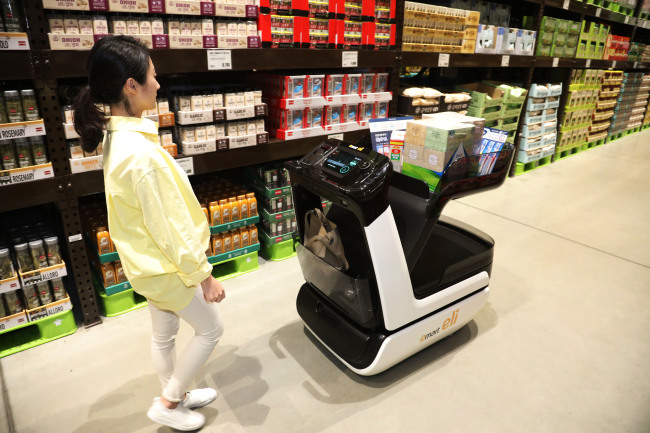
\includegraphics[width=0.48\linewidth]{figures/chap1_fig/20180417000736_0.jpg}
        \hfill
        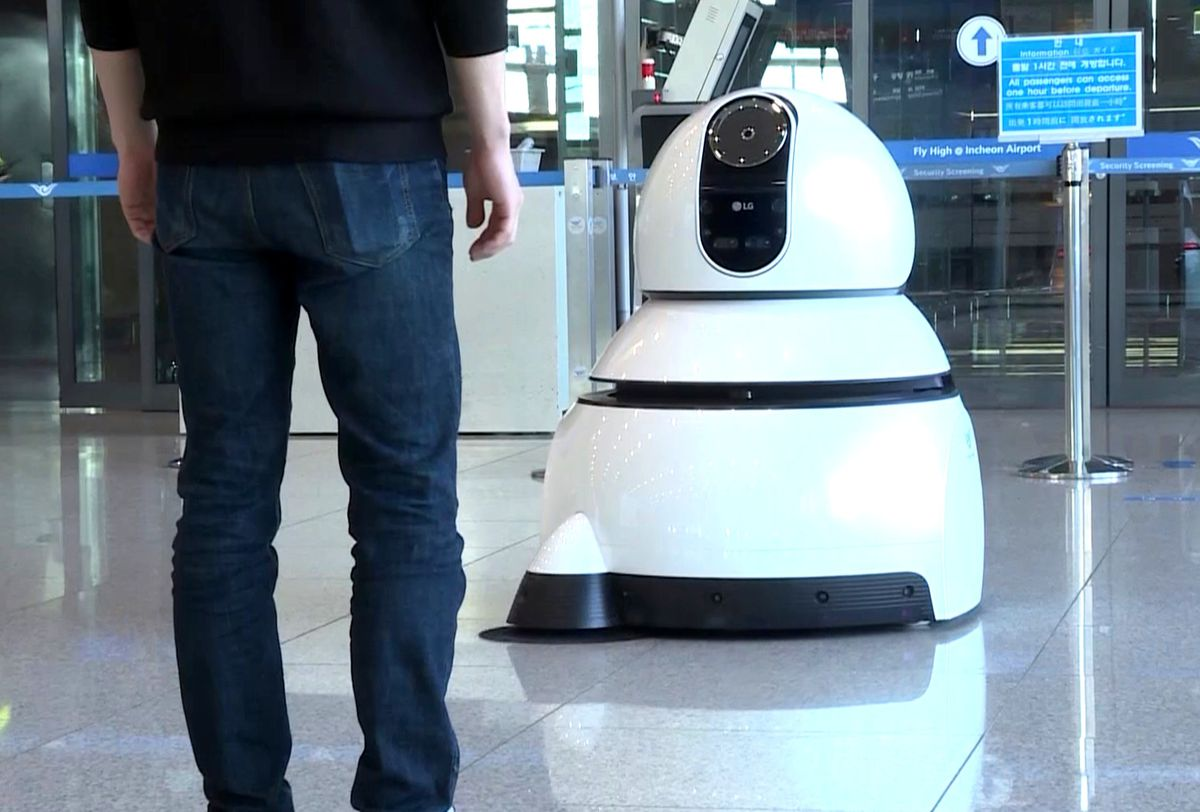
\includegraphics[width=0.48\linewidth]{figures/chap1_fig/Airport_Cleaning_Robot_02.jpg}
        \caption{Application of robot in real life\cite{intro_2,intro_3}}
        \label{Chap1:Fig1}
    \end{minipage}\hfill
\end{figure*}

Examples of applications of robots today are various, notably the application of robots to transport
goods in factories, robot vacuums, or receptionist robots with recognition
technology to assist people at airports or public areas. In addition, there are some robot applications
that follow humans to assist with specific tasks such as carrying luggage or goods (see Fig.~\ref{Chap1:Fig1}).
These systems generally use sensors to recognize information about the external environment, combined with machine learning algorithms to increase accuracy in object recognition and tracking\cite{chapter1-2}.A people following system by a robot is composed of two main modules: people identification and tracking and control to follow a recognized person.\\

\section{Research purpose}

% In this study, the focus will be on the identification and tracking of people. For previous studies, most used
In this research, we focus on identification and tracking of people. For previous studies, most used
2D LiDAR  sensors or cameras. For cameras, there are now many algorithms to identify and track people,
but for complex environments, there are still limitations such as poor visibility in weather conditions, and especially the use of cameras \cite{chapter1-3}. The field of vision is narrow, making it simple to lose the item while following and challenging to catch the right thing in time. % As for the use of 2D LiDAR, it allows identification in a wide range, can track 360 degrees, but following people in complex environments is somewhat limited because the features from 2D LiDAR  are very few, easily confused with other objects.\\
As for the use of 2D LiDAR, it allows identification in a wide range, can track 360 degrees, but following people in complex environments is limited because the features from 2D LiDAR  are very few, easily confused with other objects.\\

% Therefore, in this study, I will use 3D VLP16 LiDAR . Because 3D LiDAR  has a wide scanning range and 360 degrees
In this study, we use 3D VLP16 LiDAR . Because 3D LiDAR  has a wide scanning range and 360 degrees
like 2D LiDAR  and can capture more features like a camera. The contribution of that project is to propose a pipeline
for the robot's human tracking using 3D LiDAR.This pipeline includes two main processing parts that are user
identification online learning and control using PID controller. In addition, the pipeline will be added with
constraints and filters to increase the accuracy of identifying and following people. Moreover, using online
learning in training will boost the learning time and data since the model is continuously  updated during the
run, thereby improving accuracy and reducing data collection time from users.\\

The rest of this thesis is organized as follows.
Chapter 2 summarizes related works.
Chapter 3 presents the Human Following Robot Proposed System.
Chapter 4 details all conducted experiments and describes their results.
Chapter 5 concludes this study and states ideas for future work.
% Chapter 6 expresses the author's acknowledgments.
% Chapter 7 gives all the references used in this thesis.



